\documentclass[border=3pt,tikz]{standalone}
\usepackage{amsmath}
\usetikzlibrary{arrows}
\begin{document}
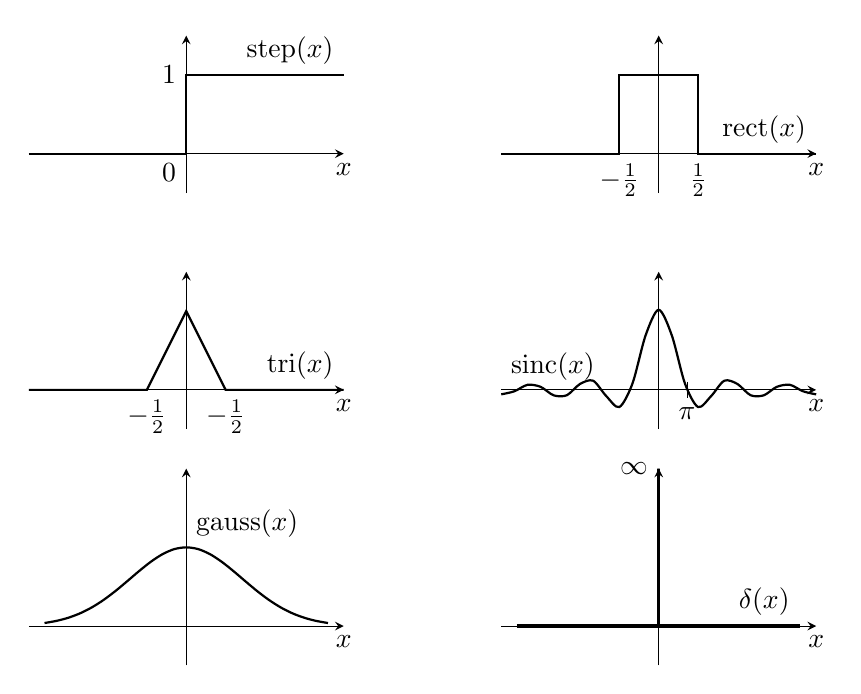
\begin{tikzpicture}[ >=stealth]


    \draw[->] (-2, 0) -- (2, 0) node[below, black] {$x$} ;
    \draw[ ->] (0, -0.5) -- (0, 1.5);
    \draw[thick] (-2, 0) -- (0, 0) node[below left, black] {$0$} -- (0, 1) node[left, black] {$1$}-- (2, 1) node[above left, black] {$\text{step}(x)$};
    
    \draw[->] (4, 0) -- (8, 0) node[below, black] {$x$} ;
    \draw[ ->] (6, -0.5) -- (6, 1.5);
    \draw[thick] (4, 0) -- (5.5, 0) node[below, black] {$-\frac{1}{2}$} -- (5.5, 1) -- (6, 1)  -- (6.5, 1)-- (6.5, 0)  node[below, black] {$\frac{1}{2}$} -- (8, 0) node[above left, black] {$\text{rect}(x)$};
    
    \draw[->] (-2, -3) -- (2, -3) node[below, black] {$x$} ;
    \draw[ ->] (0, -3.5) -- (0, -1.5);
    \draw[thick] (-2, -3) -- (-0.5, -3) node[below, black] {$-\frac{1}{2}$} -- (0, -2) -- (0.5, -3) node[below, black] {$-\frac{1}{2}$} -- (2, -3) node[above left, black] {$\text{tri}(x)$};
    
    
    \draw[->] (4, -3) node[above right, black] {$\text{sinc}(x)$} -- (8, -3) node[below, black] {$x$} ;
    \draw[ ->] (6, -3.5) -- (6, -1.5);
    \draw[domain=4.0:8.0, smooth, variable=\x, thick] plot ({\x}, {0.116*sin(500* (\x-6))/((\x-6)) -3 });
    \draw (6.36, -2.9) -- (6.36, -3.1) node[below, black] {$\pi$} ; 
    
    
    \draw[->] (-2, -6) -- (2, -6) node[below, black] {$x$} ;
    \draw[ ->] (0, -6.5) -- (0, -4);
    \draw[domain=-1.8:1.8, smooth, variable=\x, thick] plot ({\x}, {exp(-(\x)^2) - 6 });
    \node[black, right] at (0, -4.7) {$\text{gauss}(x)$};
    %\draw (6.36, -2.9) -- (6.36, -3.1) node[below, black] {$\pi$} ; 
    
    
    \draw[->] (4, -6)  -- (8, -6) node[below, black] {$x$} ;
    \draw[ ->] (6, -6.5) -- (6, -4);
    \draw[very thick] (4.2, -6) -- (6, -6) -- (6, -4) node[left, black] {$\infty$}-- (6, -6)  -- (7.8, -6) node[above left, black] {$\delta (x)$};
    
    \end{tikzpicture}
\end{document}